\documentclass{article}
\usepackage[utf8]{inputenc}
\usepackage{mathtools}



\title{\textbf{Operating Systems ID1206} \\ 
\textbf{Seminar III Report}}
\author{Emil Ståhl}
\date{December 12, 2019}

\begin{document}

\maketitle

\section{Introduction}
This report covers the implementation and testing of a green threads library written in C. The library contains its own scheduler as well as a context handler in order to handle multiple threads. In addition to this, a timer driven scheduling event will be added so that several threads can be allowed to execute concurrently. Lastly, a concurrency locking mechanism will be implemented so that race conditions can be prevented.

A thread is a subset of a process. Each process can have multiple threads executing concurrently that share all segments except the stack. Due to this, threads require mutually exclusive operations (mutexes) that will be discussed later in this report. 

\section{Managing contexts}

The managing of contexts is an important part of executing different threads on a CPU. The handler must keep track of the currently running thread as well as a set of suspended threads that are ready to be executed. A thread is therefore represented as a structure that will hold all of the information that is needed to handle this correctly. With the help of \texttt{green\_t} pointers a struct will keep track of which thread to schedule next. The threads that are dependent on other threads in order to be executed will use the field of struct \texttt{green\_t *join} that will ensure that the thread is always executed after the thread it is depended on.
However, the set of suspended threads is implemented as an ordinary FIFO queue. The queue is implemented as follows:

\clearpage
\begin{verbatim}
void add_to_queue(green_t **queue, green_t *thread_to_add) {
    
    green_t *current = *queue;    
    
    if (current == NULL) {
        *queue = thread_to_add;
    } else {
        while (current->next != NULL)	
               current = current->next;

    current->next = thread_to_add;
    }
}
\end{verbatim}
When the currently running thread has been added to the queue of suspended threads the queue is popped and the next thread up for execution is swapped with the currently running thread. 

\begin{verbatim}
swapcontext(susp->context, running->context);
\end{verbatim}{}

\subsection{Creating a thread}
A new thread is created by calling the \texttt{green\_create()} procedure. The procedure will take a \texttt{green\_t} struct to initialize, the function that shall be executed on the thread and a pointer to the arguments that should be passed to the specified function. The thread is then equipped with its own stack and the \texttt{green\_t} struct is initialized with a pointer to, among other things, the functions and its arguments. Finally, the thread is inserted into the ready queue. 

\subsection{Joining a thread}
If a thread is dependent on another thread to terminate it will use the \texttt{green\_join()} procedure. This procedure will suspend the currently running thread and add it to the queue of waiting threads. The thread will in this way be suspended until the target thread terminates. The next thread up for execution is then swapped into the CPU. 

When each thread has done its work the execution of the first joined thread begins. The memory of the terminated thread is freed as well as marked as a zombie before it is suspended in order to prevent it from being invoked by another running thread.  

\subsection{Yielding a thread}
The purpose of \texttt{green\_yield()} is to suspend the currently running thread and add it to the ready queue. The next thread up for execution is then swapped with the currently running thread. 

\section{Suspending on a condition}
The problem with the current implementation is that if a thread is given a workload that is very time-intensive the thread will not be suspended for a long time. This results in that this greedy thread is consuming all of the resources which somewhat break the concept of multithreading. To solve this the implementation is extended with conditional suspending that will suspend the currently running thread when some condition is reached. 
Conditional suspending is implemented with three procedures, which are:\\\\\texttt{green\_cond\_init(green\_cond\_t*)}
\\\texttt{green\_cond\_wait(green\_cond\_t*)}
\\\texttt{green\_cond\_signal(green\_cond\_t*)}
\\\\To put a thread to sleep the wait procedure is used and waking up a thread is done with the signal procedure.

\begin{verbatim}
void green_cond_signal(green_cond_t* cond) {

  green_t* signalled = pop_from_queue(&cond->queue);
  add_to_ready_queue(signalled);
}
\end{verbatim}

\section{Timer interrupts}
The threads have so far been able to either yield its execution or suspend on a condition. However, this is not the level of concurrency that is wanted. Each thread is executing during a time slice that is dependent on its internal behavior and workload. As a solution to this, a timer driven scheduling event is added. What this means is that when a signal is received by the process the currently running thread will be suspended even thus it has not completed its work. However, there is no need to reinvent the wheel. When the signal is received by the process it is told to execute the \texttt{timer\_handler()} procedure which in turn calls the \texttt{green\_yield()} procedure. All threads will now operate during a fixed and fair time slice that easily can be specified in the code. 

\subsection{Blocking interrupts}
The problem with this implementation is that if a timer interrupt is received in the middle of a yield operation or other functions that manipulates the green threads. These interrupts are therefore prevented from being received when a thread is being enqueued or dequeued. 

\begin{verbatim}
sigprocmask(SIG_BLOCK, &block, NULL);
add_to_ready_queue(new);
sigprocmask(SIG_UNBLOCK, &block, NULL);
\end{verbatim}

\section{Concurrency control}
Since a thread now can be interrupted at any point in the execution there will arise race conditions when two threads update a shared counter. The implementation is therefore once extended, this time with mutual exclusion locks. The procedures that will take care of this are: \texttt{green\_mutex\_init()}, \texttt{green\_mutex\_lock()} and \texttt{green\_mutex\_unlock()}. The locking mechanism works as follows: 

\begin{verbatim}
int green_mutex_lock(green_mutex_t* mutex) {
  
  sigprocmask(SIG_BLOCK, &block, NULL);
  green_t* susp = running;
  
  while(mutex->taken) {
  
    add_to_queue(&mutex->susp, susp);
    set_next_running(); 
    swapcontext(susp->context, running->context);
  }
  mutex->taken = TRUE;
  sigprocmask(SIG_UNBLOCK, &block, NULL);
  
  return 0;
}
\end{verbatim}
When the locking procedure is called the status of the lock will be checked and if taken the thread that initiated the call will be added to the queue of suspended threads and yielded. Otherwise, the taken pointer field will be set to TRUE and the thread now holds the lock. Upon releasing the lock all threads that were suspended are added back to the ready queue.

\section{Benchmarking}
For all benchmarking in this report, a benchmarking program written in C will be used. The program will start two threads which are set to execute a function \texttt{test()}. This procedure will make one of the threads a producer and the other will act as a consumer. The two threads will take turn updating a global variable \textbf{buffer}, the producer will set the value to 1 and the consumer will set the value to 0. Each thread will perform this 20.000 times before terminating. 

However, in order to prevent race conditions while manipulating the shared buffer the threads will utilize mutex locks before entering the critical section. In addition to this, while the threads are waiting for the other one to do its job they will be put to sleep with the call to \texttt{cond\_wait(\&cond, \&mutex)} along with a condition to wait for. 
When a thread is done updating the \textbf{buffer} it will make a call to \texttt{cond\_signal(\&cond, \&mutex)} in order to wake up the thread waiting on this condition. Lastly, the mutex lock is released. 
This benchmark is performed both with the green threads library described earlier in this work as well as with the built-in POSIX threads library. The results are presented in the figure below.

\begin{figure}[h]
\centering
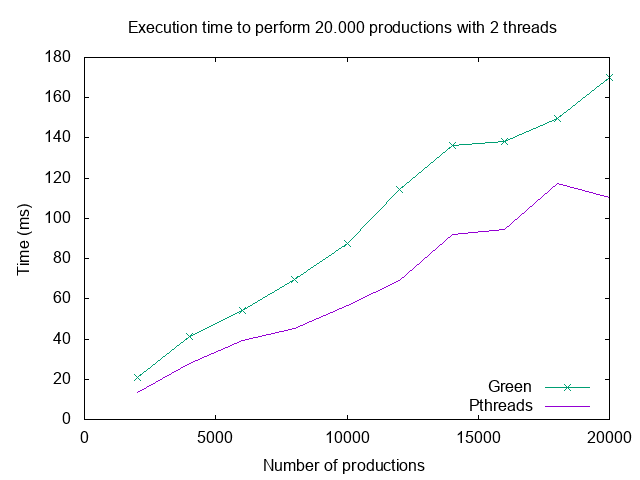
\includegraphics[width=1.0\textwidth]{multi.png}
\caption{Benchmarking of green threads compared to POSIX threads}
\end{figure}

\section{Main problems and solutions}
This section will focus on the problems that were encountered during the work and how they were solved. 

\subsection{Implementing the ready queue}
To implement a queue to hold the threads that are suspended on a condition a new structure called \texttt{green\_cond\_t} was created that holds a \texttt{green\_t *queue} data type which consists of all of the pointer fields of the \texttt{green\_t} struct. As always when working with pointers in C there will arise tricky bugs that are not that easy to solve. A good amount of time was spent on figuring this out. 

\subsection{When to unlock?}
Mutex locks are for sure a powerful tool which needs to be done carefully to avoid deadlock. The tricky part of this work was to figure out when to release the lock. When a thread is put to wait on a condition, the lock is released before the thread is enqueued. This required some effort to understand what was going on. 

\subsection{Working with conditional variables}
One of the most struggling parts of this work was to grasp the concept of conditional variables. The hardest part to understand was that the condition is just that, a condition. However, things started to get much clearer upon working with the concept while writing the test program.

\subsection{Where to wake up?}
Another mind-boggling concept of this work was to find out where a thread wakes up after having been suspended by the timer interrupt. Interestingly, when the suspended thread is scheduled again it will continue the execution from the point where it was put to sleep which is immediately after the \textbf{swapcontext()} system call. Even thus this is a reasonable concept it was not that clear in the beginning of this work. 


\section{Summary}
This work has focused on implementing a green threads library that runs in user space. The main topics covered was to better understand the advantages and problems that a multithreaded system results in. Three primary areas were covered. The first part covered was to manage contexts and threads. Secondly, conditional suspending was evaluated and implemented. In order to run several threads concurrently the implementation was extended with a timer interrupt. Lastly, in order to prevent race conditions concurrency control was added. However, this work required a deep understanding of many different concepts and resulted in very laborious debugging. Consequently, it was a very interesting and educative experience that probably will turn out to be useful in future work. 


\end{document}
